% The layout of your thesis is fairly flexible, so don't feel you need to follow the chapters
% in this template. It's a good idea to talk through your structure with friends and your 
% supervisor to check it is logical and flows to someone with little understanding of the content.
%
% Here is a brief outline of the structure of each chapter:
%  1. Introduction
%      - First paragraph should link this chapter to the previous chapter(s) and overall progress
%      - Follow this by stating the aim and function of this chapter (what does it add to your 
%        overall argument?). Make sure the reader knows what they should get out of it.
%      - Provide an overview of how you'll do that (perhaps what each section adds to the argument)
%  2. Body
%      - This is mostly up to you. Before you start writing make sure you WRITE DOWN what the main
%        content points and arguments are. Structure your sections in a logical way around these.
%      - Feel free to begin with a "Fundamentals" section, or weave this into the start of 
%        individual sections to provide (necessary) technical background to the areas you work in
%  3. Conclusion
%      - Don't just summarise what you did, state the significance and implications of what you found.
%      - Only state conclusions which can be made from this chapter alone. Leave the overall argument
%        and main conclusions for the Discussion and Conclusion chapters.
%
% A couple of tips:
%  - I always found it helpful to start with a few levels of dot-points (OneNote, Google Docs, Word)
%    to get the content down. Then you can easily see where it is lacking, and you can rearrange it
%    quickly to get a better structure and flow. Remember the reader understands a LOT less about this
%    than you do, so good explanations are important!
%  - Don't be afraid to start writing. Even if you think it will be garbage. Even if you're not
%    completely sure what to say. Just start. The action of writing it out will clarify your argument
%    in your own mind and help you with development. You also get to see where there is room for 
%    improvement in your argument. I wrote most of my chapters 3 times and each time it became a lot 
%    more logical and I was a lot happier with it. While I spent a more time writing, it saved me a 
%    lot of time procrastinating and wondering how to write it perfectly first time.

\chapter{Methodology}
\label{cha:methodology}

With the scope of the work now defined, the manner in which the required results will be obtained can now be detailed. The necessary additions as defined in Section \ref*{sec:intro_scope}, Scope, may will be implemented in the form of two independent assemblies in order to meet the requirements of the work. These two assemblies will be refereed to as the Processor Module and the Magnetic Separation Station. The former will be the site of the chemical reactions as described in Section \ref{subsec:intro_extraction}, The Extraction Process, and will be the hardware element that forms the SBS block on the Gene-Plex Extractor deck. Therefore, given it will house the full set of reactions, it will also encompass the software and hardware requirements of the liquid temperature control (including the associated controller), along with the magnetic separation required in tube number 4 of the cassette. The Magnetic Separation Station will be the location of disposal of the supernatant and therefore shall include the magnetic hardware required to physically manipulate the magnetic silica beads in order to retain them in the pipette tip while the waste is expelled. Given the biological nature of the liquid waste involved, this station will also include provisions for hygienically disposing of and storing this waste.

\section{Processor Module}

\subsection{Hardware}

The hardware component of the Processor Module design is concerned with ensuring the module accepts the required cassette tubes, fits within the stipulated SBS space and provides a stable platform for the required temperature control using the knowledge gained in Section \ref{lit_controlability}, Controllability. The work in this sections will also include the selection of an appropriate heat pumping device. In order to ensure the requirements of the hardware elements are met, the design process is applied as follows:
\begin{enumerate}
	\item Generation of concepts related to thermally isolating the heated and non-heated regions of the block. This includes a focus on the manufacturability of the resulting components.
	\item Investigation into and selection of an appropriate heating method.
	\item Full CAD design of hardware including provisions to accommodate the required tubes.
	\item Utilization of 3D printing to test the fit of the cassette tubes in the block design.
	\item CFD simulation to verify the performance of the selected heating element and the thermal stability of the final design. 
\end{enumerate}

\subsection{Temperature Controller}

This work will output a software temperature controller capable meeting the liquid heating requirements of the chemical reaction as detailed in Section \ref{subsec:intro_extraction}, The Extraction Process. The following method is followed to ensure the desired output is obtained:
\begin{enumerate}
	\item Assembly of the fully manufactured Processor Module.
	\item Utilize sensors in the locations given in below to gather data of the temperature at relevant points over time:
	\begin{itemize}
		\item The temperature at the centre of the block will be taken as this sensor data is what will be used as feedback for the controller to be implemented. This follows the recommendations given in Section \ref{cha:literaturereview} by Vilchiz et. al.
		\item The temperature of the heatsink will be plotted to monitor the temperature differential created across the module if TEC's are selected as the heat pump device.
		\item The temperature of the heated region of the module will be taken on its outer surface to determine the success of the design in creating a component that responds to temperature control in responsive and stable manner.
		\item The temperature of the liquid within the cassette tubes will be measured as the final output of the system. The ability of the controller to drive this temperature to the desired set point will determine the success of the design.
	\end{itemize}
	\item An Arduino will be used as an interface device to connect to MATLAB, which will be used as a data logger and analysis tool. The real time data will be displayed along with stored for future use.
	\item The software and electronics used to control the MTX Cycler (see Section \ref{sec:intro_scope}) will be modified to provide a step input to the system.
	%ADD DETAILS FOR CONTROLLER DESIGN HERE
	\item The response of the system to the step input will then be logged and the temperature response of the block centre will be used to identify the modules plant function via MATLAB.
	\item A Simulink simulation will then be created to validate the estimated system parameters produce an output which matches the response obtained experimentally.
	\item A discrete controller will then be designed via the direct method.
	\item The designed controllers ability to drive the system to a steady state of 60$\degree$C with then be validated via Simulink simulation.
	\item  The validated controller will then be implemented via the MTX Cycler software with any required modifications.
\end{enumerate}

\subsubsection{Experimental Verification}

In order to verify the performance of the resulting controller, the following experimental verification will be conducted. The experiment will determine the ability of the controller to meet the steady state error, disturbance rejection, response time, overshoot and stability requirements when controlling temperature in the module. The method is as follows:

\begin{enumerate}
	\item Assemble 4 complete Processor Modules
	\item Using an Arduino as an interface and MATLAB as the data logger and analyser, measure the temperature in the tubes shown in Figure \ref{fig:measuredtubes} for the duration of the experiment.This distribution will allow the performance at the extremes of the device to be determined.
	\begin{figure}[!htb]
		\centering
		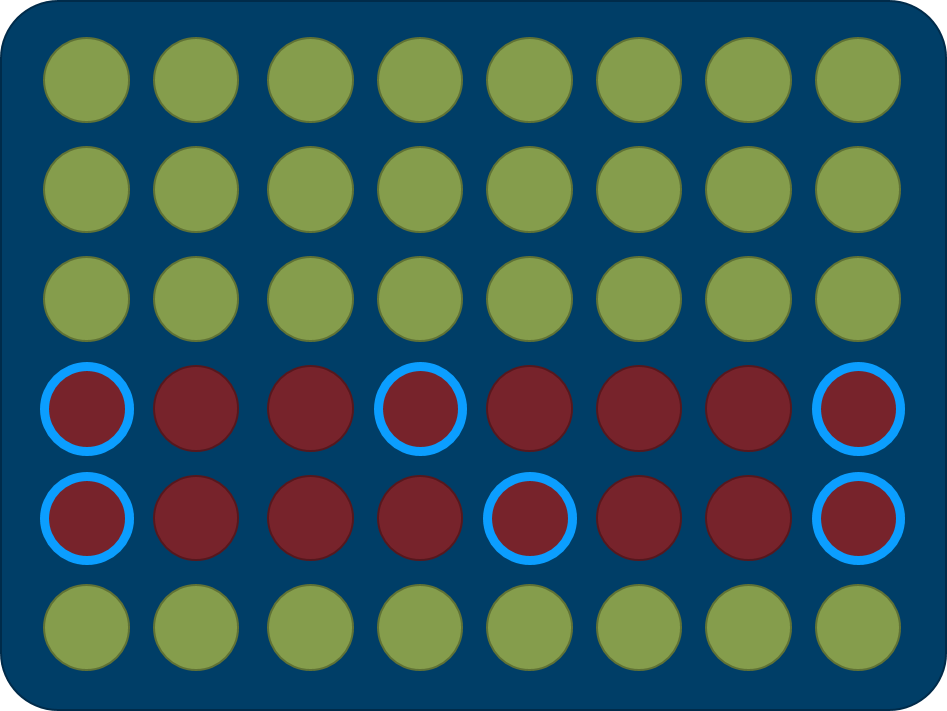
\includegraphics[width = \textwidth]{measuredtubes.png}
		\caption[Temperature Measured Tubes.]{Tube locations to be measured during temperature control verifications experiment. Non-Heated tubes are coloured green, heated tubes are coloured red, measured tubes are outlined in blue.}
		\label{fig:measuredtubes}
	\end{figure}ˆ 
	\FloatBarrier
	\item Begin data logging and live plotting.
	\item Set the reference input to the controller to 60$\degree$C.
	\item Collect data for a total of 30 minutes to capture the long term steady state performance of the module (to allow any slow heat transfers to be observed) along with the transient response.
	\item Repeat the experiment for all four assembled modules. This allows for the controllers ability to reject disturbances caused by the differing of the plant properties to be determined as is caused by the slight differences in assembly.
	\item Repeat experiment in differing environmental conditions. The experiment should  be conducted in rooms at temperatures of 18$\degree$C, 22$\degree$C and 26$\degree$C. This allows for the disturbance rejection of the controller to be assessed where the disturbance is due to altered environmental conditions.
	\item Use the collected data to assess the consistency of the heating profile and the temperature stabilisation across the tubes of the module. These results will be used to make conclusions regarding the designed controller along with the thermal characteristics of the hardware. It should be noted that the worst case response will be used to draw conclusions regarding performance to ensure all samples fall within the requirements.
\end{enumerate}

\subsection{Magnetic Separation}

As the final stage of the extraction process is the removal of the clean sample from the waste beads, the success of extraction depends on the complete and reliable separation in tube number 4. To ensure this is achieved, the following design process and experimental verification will be conducted:
\begin{enumerate}
	\item An investigation will be conducted into the various possible methods of magnetic separation in this application, taking into account the recommendations to use ND-Fe-B magnet compositions as found in the reviewed literature.
	\item 3D Printed test jigs will be created to test the effectiveness of the most suitable configurations via manual inspection.
	\item With a preferred design selected, the a test module will be 3D printed including the magnetic arrangement. This test module will be assembled on the robot deck and verified experimentaly via the method described below.
\end{enumerate}

\subsubsection{Experimental Verification}

To allow a confident conclusion to be made regarding the effectiveness of the magnetic separation within the Processor Module to be made, the following experiment will be conducted. This experiment will replicate the setup used by the robot and its processes to ensure the result is representative of the true scenario.

\begin{enumerate}
	\item Place test module with magnetic separation on Gene-Plex Extractor deck within one of the SBS spaces.
	\item Place a 5mL tube on the robot deck to collect the experiment output.
	\item Place a full set of 8 cassettes in the test module with 100$\mu$L of filtered water and 10$\mu$L of magnetic beads in tube 3. The water will simulate the elution buffer. Both volumes are equal to that used in the final process.
	\item Instruct the robot to aspirate the mixture in tube 3 and expel it into tube 4, the location of the magnetic separation.
	\item Wait for 5 seconds for separation to take place. It should be noted that this waiting period is a design variable and may be adjusted and this experiment repeated to determine the optimal wait time.
	\item Aspirate the separated liquid at a distance of 1mm from the tube bottom. This distance once again may be adjusted, however is a sound starting point for experimentation.
	\item Expel the liquid from the tip into the 5mL tube on the deck.
	\item Repeat this separation procedure for all 8 cassettes.
	\item Refill all cassettes with equal volumes of water and beads, as was defined in step 3.
	\item Repeat the separation for a total of 3 modules to equal the total volume of liquid which will be processed by the Gene-Plex Extractor during the processing of all 24 samples.
	\item Place the 5mL tube with extracted contents adjacent to a large ND-Fe-B magnet to draw any beads to the tube wall. Examine the tube contents for any sign of magnetic beads. The presence of a bead within the tube indicated a failed separation within tube 4. Such a result may lead to severe complications in step 2 (amplification), such as the failed diagnosis of a patient. Therefore, for a successful verification, it is required that no beads are present.
\end{enumerate}

\section{Magnetic Separation Station}

The magnetic separation station is a standalone module on the robot deck which will fulfil two requirements of the extraction process. Firstly, the station will provide the means of separating the waste liquid from the magnetic beads and captured DNA/RNA, as necessary after step 2 (refer to Section \ref{subsec:intro_extraction}) of the extraction process. Following the successful separation of the supernatant, the separation station will provide a means of hygienically disposing of the associated biological waste. The work will be completed via the the methodology described below.

\subsection{Magnetic Separation}

This stage of the extraction process carries a high level of significance in relation to the final result. Poor magnetic separation may effect the reliability of the diagnosis due to a reduction in the sensitivity of the step 2 amplification, or failure of step 3 analysis due to the presence of inhibitors. The former may be caused by a lack of concentration of the target DNA or RNA in the extracted clean sample. Failed magnetic separation could cause this by not properly capturing the magnetic beads and bound target, allowing them to be expelled into waste. This loss of target will lower the sensitivity of the amplifications stage and hence may lower the accuracy of diagnosis. The second scenario of inhibitors may occur if some of the waste liquid remains after washing, contaminating the sample and lowering the effectiveness of the amplification and analysis steps. Therefore, the method used for the design of the magnetic separation capabilities of the Magnetic Separation Station is aimed at ensuring a strong and reliable separation.

\begin{enumerate}
	\item An investigation will be carried out to determine the most suitable magnetic arrangement for providing reliable separation. Similar to the treatment of the magnetic separation capabilities within the Processor Module, the investigation will focus on those employing the ND-Fe-B composition.
	\item The selected configuration will then be implemented as a design concept and a CAD model generated. This detailed design will also account for a number of secondary requirements. These include maintaining a minimum distance between the pipette tip and the Separation Station at all points to remove the possibility of cross contamination occurring through liquid transfer.
	\item The detailed design will then be prototyped using 3D printing to allow experimental verification.
	\item The prototype Separation Station will then be assembled on the Gene-Plex Extractor deck along with the necessary tubes to perform magnetic separation via the experimental procedure detailed below.
\end{enumerate}

\subsubsection{Experimental Verification}

In order to verify the required performance is achieved by the designed Magnetic Separation Station, the following experiment will be performed.

\begin{enumerate}
	\item The prototyped Magnetic Separation Station will be fully assembled and positioned on the deck of the Gene-Plex Extractor.
	\item 3 cassettes and therefore 24 tubes will be positoned on the deck with 640$\mu$L of water and 10$\mu$L of magnetic silica beads in each. These volumes are equal to those used in the extraction process and this will be repeated 24 times, once for each of the 24 samples. Therefore, this setup matches the volumes to be processed by the implemented extractor.
	\item The robot will then be setup to aspirate the liquid mixture from one of the tubes.
	\item The pipette will then be positioned within the magnetic separation station and lowered to full depth. 
	%NOTE THAT A DIAGRAM OF THIS WOULD BE GOOD to show positions
	\item The pipette tip will then be raised and lowered with the full liquid height passing along the magnetic arrangment a total of 2 times.
	%DETERMINE THESE DISTANCES AND PUT IN DIAGRAM
	\item With the beads now separated from the liquid and captured on the pipette wall, the water will be ejected into the waste disposal system. For this experiment, the waste disposal will be replaced by a small glass container that may be used to collect and analyse the ejected liquid.
	\item This procedure will then be repeated for all 24 ``samples".
	\item The contents of the waste container will then be subjected to a magnetic field to collect any beads which were not correctly separated by the process. The presence of any bead within the waste liquid indicated a failed separation.
	%ADD PERCENTAGE TOLERANCES OR VOLUMES 
\end{enumerate}

\subsection{Waste Disposal}

The work on this component of the Magnetic Separation Station is concerned with ensuring the product meets key standards and requirements in order to dispose of the biological waste in a hygienic manner. The disposal of the waste generated by the process is a key factor in ensuring a successful sample extraction. Any failure to safely dispose of this waste may introduce the risk of a cross contamination occurring between two independent samples and therefore a failure to correctly diagnose the patient.\\

To ensure the waste disposal system negates these risks, the process used will focus on researching the related standards initially in order to determine the best practices which must, by regulation, be adhered to. This research will be supplemented by end user feedback. To gain this, a group of key product users will be consulted on preferred methods of waste disposal and hygiene to guide the design process. Using the results of this investigation, the design process will be used to form a final design which takes into account the gathered information and requirements and therefore produce a functional and hygienic waste disposal system.